%----------------------------------------------------------------------------------------
%    ONES
%----------------------------------------------------------------------------------------
\section{Ones}
\begin{itemize}
    \item Moviment ondulatori: transporta $\begin{cases} E \text{ (energia)} \\ \vec{P} \text{ (moment lineal)} \\ \vec{L} \text{ (moment angular)} \end{cases}$
    \item Tipus:
        \subitem Mecàniques: requereixen medi.
        \subitem Electromagnètiques: no requereixen medi.
\end{itemize}

\subsection{Característiques}
\begin{itemize}
    \item Focus emissor: origen de la pertorbació. Aporta energia.
    \item Material: les forces intermoleculars són les responsables de la propagació de l'ona: $v_{p} \propto F_{\text{int}}$; en ones electromagnètiques, $v_{p} = c$.
    \item Tipus d'ones:
        \subitem Transversals: la pertorbació és perpendicular a $v_{p}$.
        \subitem Longitudinals: la pertorbació és paral·lela a $v_{p}$.
    \item Front d'ona:
        \subitem Ona esfèrica:
        \subitem Ona plana:
    \item Magnituds:
        \subitem Velocitat de propagació: no depèn del focus i és $\perp$ als fronts d'ona. $\boxed{v_{p} = \frac{\partial x}{\partial t}}$, $\boxed{v = \lambda \nu}$.
        \subitem Freqüència: $\boxed{\nu = \frac{1}{T}}$.
        \subitem Freqüència angular: $\boxed{\omega = 2 \pi \nu}$.
        \subitem Nombre d'ones: $\boxed{k = \frac{2 \pi}{\lambda}}$.
\end{itemize}

%----------------------------------------------------------------------------------------
\subsection{Equació d'ona}
La velocitat de propagació d'una ona en una corda oscil·lant és:
\begin{align}
    \boxed{v_{p} = \sqrt{\frac{T}{\mu}}}
\end{align}
on $T \equiv$ tensió de la corda i $\mu \equiv$ densitat lineal de la corda.
\begin{align}
    \boxed{\frac{\partial^{2} y}{\partial t^{2}} = v_{p}^{2} \frac{\partial^{2} y}{\partial x^{2}}}
\end{align}

%----------------------------------------------------------------------------------------
\subsection{Ones viatgeres}
Compleixen l'equaciçó d'ones aquelles ones tal que:
\begin{align}
    \boxed{f(x,t) = f(x \mp v t)}
\end{align}
\begin{figure}[H]
\centering
    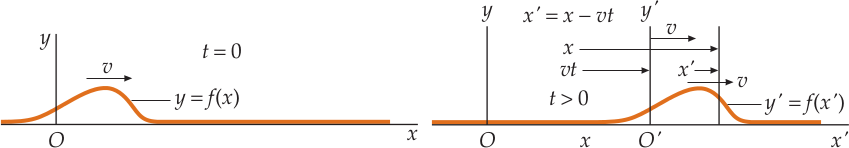
\includegraphics[width=\textwidth]{images/2/23-viatgeres.png}
\caption{Pols de corda en moviment. Es compleix que $x' = x - vt$}
\end{figure}

%----------------------------------------------------------------------------------------
\subsection{Ones harmòniques}
\begin{align}
    \boxed{\psi (x,t) = \psi_{0} \sin (x \mp v t)}
\end{align}
\begin{align}
    \boxed{y (x,t) = A \sin (kx - \omega t)}
\end{align}
\begin{figure}[H]
\centering
   %\def\svgwidth{\columnwidth}\input{./images/2/2-2-harmoniques.pdf_tex} 
   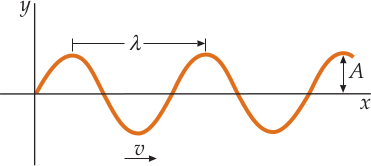
\includegraphics[width=0.5\textwidth]{images/2/24-harmonica.png}
\caption{Representació gràfica d'una ona harmònica en funció de $x$. Es compleix que $\lambda = v T$}
\end{figure}

\subsubsection*{Energia (en una corda)}
\begin{align}
    \boxed{\Delta E = \frac{1}{2} k_{m} A^{2}} \qquad \text{on } k_{m} = m \omega^{2}
\end{align}
\begin{align}
    \Delta E = \frac{1}{2} \mu v \Delta t \omega^{2} A^{2} \Rightarrow \boxed{P_{m} = \frac{1}{2} \mu v \omega^{2} A^{2}}
\end{align}
\subsubsection*{Diferència de fase}
Sigui $\psi (x,t) = \psi_{0} \sin (\omega t \pm kx \varphi_{0})$. Llavors definim la diferència de fase com:
\begin{align}
    \boxed{\Delta \varphi = \varphi_{2} - \varphi_{1}}
\end{align}
\begin{itemize}
    \item Per a temps $t$ fix:
        $\begin{gathered} \boxed{\Delta \varphi = k \Delta x = \frac{2 \pi}{\lambda} \Delta x}. \end{gathered}$
    \item Per a posició $x$ fixa:
        $\begin{gathered} \boxed{\Delta \varphi = \omega \Delta t \ = 2 \pi \nu \Delta t}. \end{gathered}$
\end{itemize}
Quan tenim dues ones harmòniques, $\forall m \in \mathbb{N}$, les dues ones estaran:
\begin{itemize}
    \item En fase: $\boxed{\Delta \varphi = 0 \pm 2 \pi m}$.
    \item En contrafase: $\boxed{\Delta \varphi = (2m \pm 1) m}$.
    \item En quadratura: $\boxed{\Delta \varphi = (\frac{1}{2} + m) \pi}$.
\end{itemize}

%----------------------------------------------------------------------------------------
\subsection{Principi de superposició lineal}

%----------------------------------------------------------------------------------------
\subsection{Interferències}
\subsubsection*{Ones estacionàries}
\subsubsection*{Ones harmòniques}
\subsubsection*{Polsació d'ones}
\subsubsection*{Patrons d'inteferència}
\begin{figure}[H]
\centering
    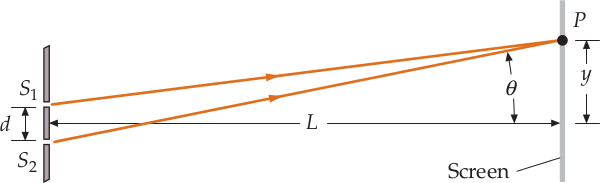
\includegraphics[width=0.8\textwidth]{images/2/26-doble-escletxa.png}
\caption{Diagrama de patró d'inteferències de doble escletxa a una paret. Les distàncies entre elles són $y_{n}$, on $n$ és l'ordre d'interferència}
\end{figure}
\begin{align}
    \boxed{y_{n} = \frac{x \lambda}{d} n}
\end{align}
\subsubsection*{Diferents eixos de vibració}
\begin{figure}[H]
\centering
    WIP: GRAFIC BONIC 
\caption{Figures de Lisajous, la resultant de la superposició és una ona polaritzada}
\end{figure}
\subsubsection*{Difracció}
\begin{figure}[H]
\centering
    WIP: GRAFIC BONIC 
\caption{Difracció d'una ona en una escletxa}
\end{figure}
%----------------------------------------------------------------------------------------
\subsection{Intensitat}
\begin{align}
    \boxed{I = \frac{\Delta E}{\Delta S \Delta t}} \quad \left[ \si{\W\per\m\squared} \right]
\end{align}

\subsubsection*{Mesura de la intensitat}
El rang de $I$ audibles pels humans és $\begin{cases} I_{max} = \SI{1}{\W\per\m\squared} \\ I_{min} = \SI{10 e-12}{\W\per\m\squared} \equiv I_{0} \end{cases}$

Així doncs, definim el nivell d'intensitat com:
\begin{align}
    \boxed{\beta = 10 \log \left( \frac{I}{I_{0}} \right)} \quad [\si{\dB}]
\end{align}

\subsubsection*{Atenuació per propagació}
\begin{itemize}
    \item Circulars: $\begin{gathered} \boxed{I(r) = \frac{I_{0}}{2 \pi r}} \end{gathered}$.
    \item Esfèriques: $\begin{gathered} \boxed{I(r) = \frac{I_{0}}{4 \pi r^{2}}} \end{gathered}$.
\end{itemize}

\subsubsection*{Intensitat en dues dimensions}
\begin{align}
    \boxed{I = \frac{1}{2} \mu v \omega^{2} \frac{A^{2}}{\Delta S}}
\end{align}

\subsubsection*{Intensitat en tres dimensions}
\begin{align}
    I = \frac{1}{2} \rho \omega^{2} s_{0}^{2} v; \quad s_{0} = \frac{p_{0}}{\rho \omega v} \Rightarrow \boxed{I = \frac{1}{2} \frac{p_{0}^{2}}{\rho v}}
\end{align}

%----------------------------------------------------------------------------------------
\subsection{Efecte Doppler}
\begin{figure}[H]
\centering
    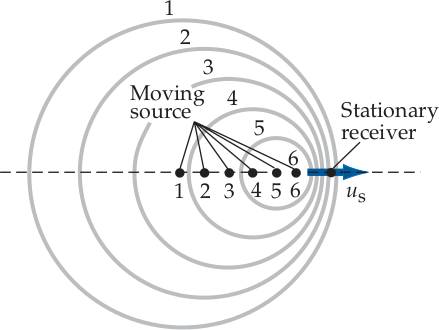
\includegraphics[width=0.5\textwidth]{images/2/28-doppler.png}
\caption{Diagrama de l'efecte Doppler per a un emisor $E$ i un receptor $R$ amb una velocitat relativa entre l'un respecte l'altre}
\end{figure}
\begin{align}
    \boxed{\nu_{r} = \frac{v_{p} \pm u_{r}}{v_{p} \mp u_{e}} \nu_{e}}
\end{align}

\subsubsection*{Criteri de signes}
\begin{itemize}
    \item $\begin{gathered} \frac{+}{-} \end{gathered}$: aproximació E-R $\Rightarrow \nu_{r} > \nu_{e}$.
    \item $\begin{gathered} \frac{-}{+} \end{gathered}$: allunyament E-R $\Rightarrow \nu_{r} < \nu_{e}$.
\end{itemize}
Observació: el medi trenca la simetria: $E \to R \neq R \to E$.
\subsubsection*{Ones de xoc}
\begin{figure}[H]
\centering
    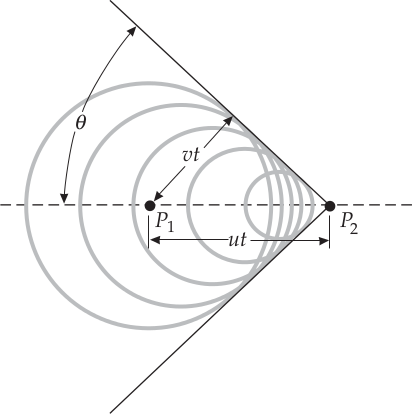
\includegraphics[width=0.5\textwidth]{images/2/28-ones-xoc.png}
\caption{Situació en què es produeixen ones de xoc}
\end{figure}
\begin{align}
    \boxed{\sin \theta = \frac{v}{u} = \text{(Nre. Mach)}^{-1}}
\end{align}

\subsubsection*{Efecte Doppler relativista}
\begin{align}
    \boxed{\nu_{r} = \nu_{e} \sqrt{\frac{1 \pm \beta}{1 \mp \beta}}} \qquad \text{on } \beta = \frac{v_{rel}}{c}
\end{align}
Té el mateix criteri de signes.
%----------------------------------------------------------------------------------------
\subsection{Propagació del so}
\begin{itemize}
    \item Líquids i sòlids: $\begin{gathered} v_{\text{so}} = \sqrt{\frac{B}{\rho}} \end{gathered}$.
    \item Gasos: $\begin{gathered} v_{\text{so}} = \sqrt{\frac{\gamma RT}{M}} \end{gathered}$.
\end{itemize}
